\section{Convolution}
\label{sec:convolution}


\begin{center}%
\begin{figure}
\begin{centering}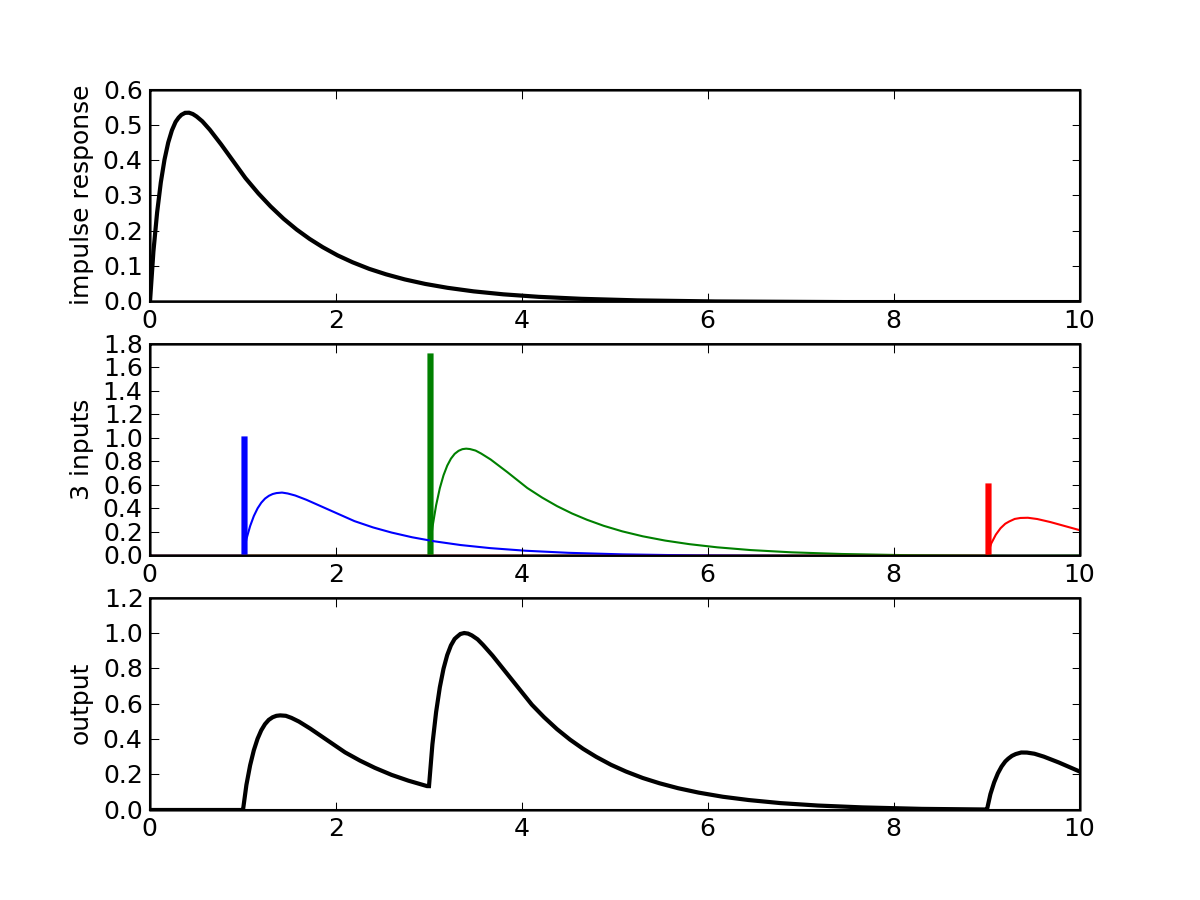
\includegraphics[width=4in]{fig/convolve_explain}\par\end{centering}
\caption{\label{fig:convolve_explain}The output of a linear system to a series of impulse inputs is equal to the sum of the scaled and time shifted impulse response functions.}
\end{figure}
\par\end{center}

\begin{center}%
\begin{figure}
\begin{centering}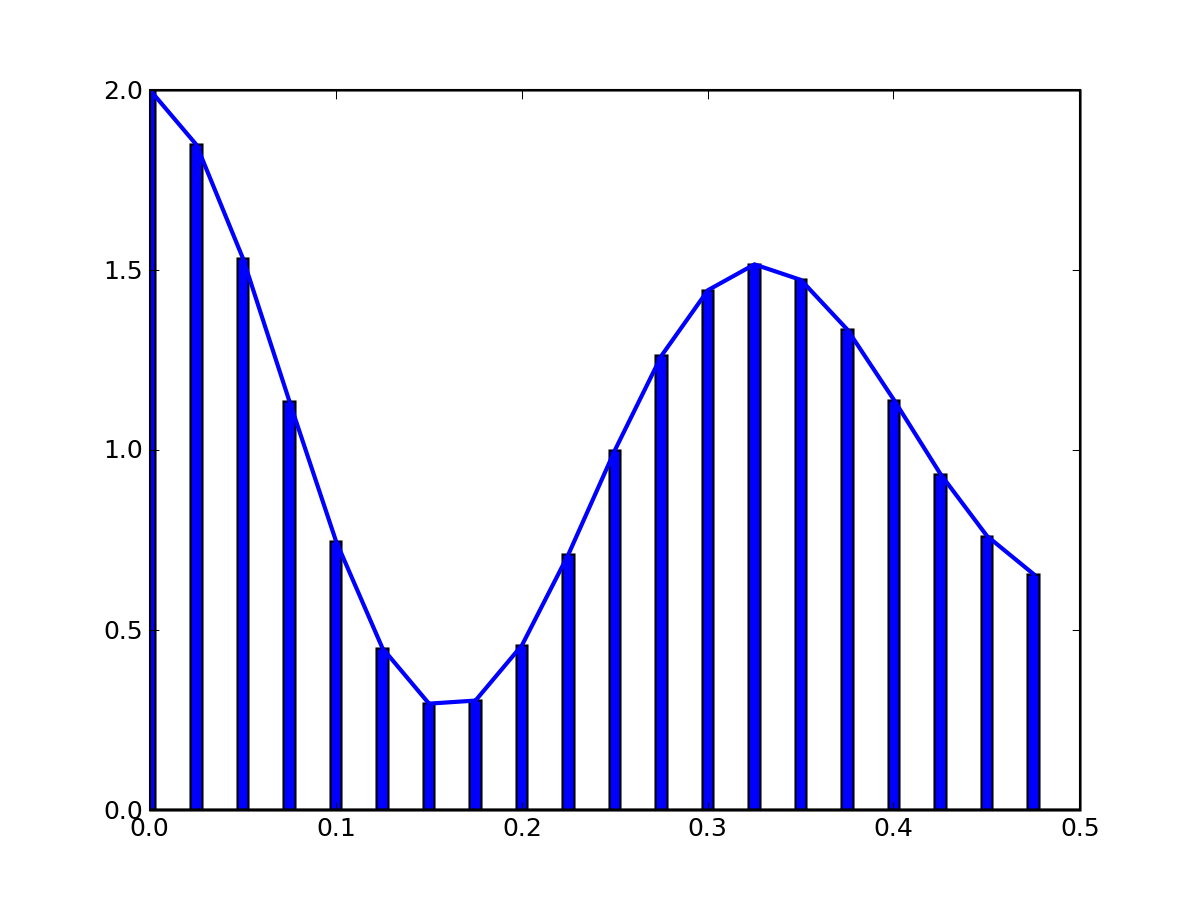
\includegraphics[width=4in]{fig/convolve_deltas}\par\end{centering}
\caption{\label{fig:convolve_deltas}Representing a continuous time signal sampled as a sum of delta functions.}
\end{figure}
\par\end{center}


\lstinputlisting[label=code:convolution_demo,caption={IGNORED}]{skel/convolution_demo_skel.py}



\begin{center}%
\begin{figure}
\begin{centering}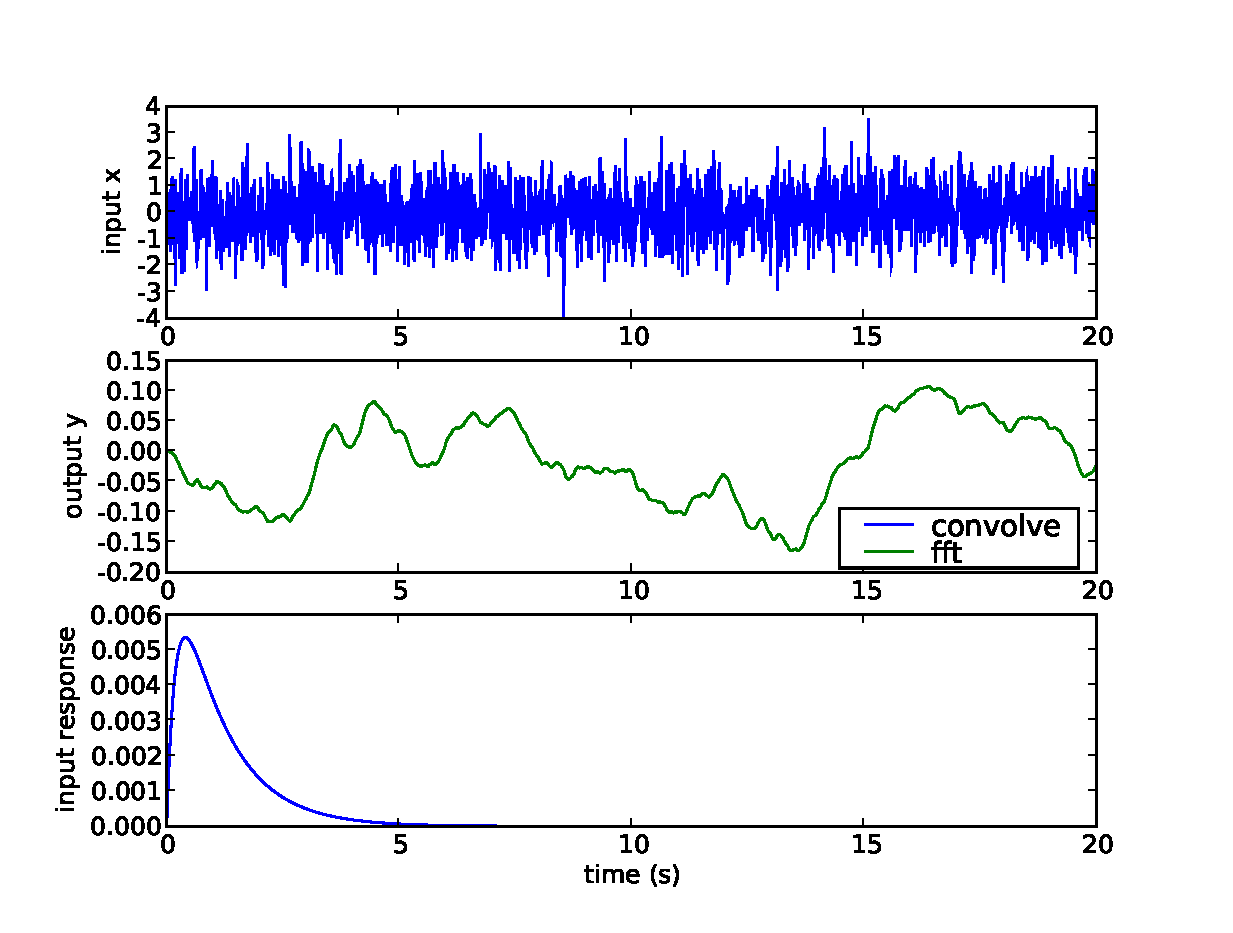
\includegraphics[width=4in]{fig/convolution_demo}\par\end{centering}
\caption{\label{fig:convolution_demo}Convolution of a white noise process with a double exponential function computed with \texttt{numpy.fft} and \texttt{numpy.convolve}}
\end{figure}
\par\end{center}
